\documentclass[english]{article}

\usepackage{babel}
\usepackage{graphicx}
\usepackage{times}
\usepackage{pifont}
\usepackage[margin=1in]{geometry}
\usepackage{eurosym}
\usepackage{fancyhdr}
\usepackage[hidelinks]{hyperref}
\usepackage{listings}
\usepackage{color}
\usepackage{float}

\pagestyle{fancy}
\fancyhf{}


%HEADER
%**************************************************************************************
\pagestyle{fancy}
\fancyhf{}
%**************************************************************************************
\lhead{Atmel Studio 6}		 	 
\rhead{Basics of Microprocessor technology} 
\lfoot{EFA12SF}
\cfoot{\thepage}
\rfoot{Nikolay Arsenov\\Alexey Tukalo}
%**************************************************************************************

\date{}
\setlength\parindent{0pt}

\begin{document}

\title{\vspace{2in}    Atmel Studio 6\\
\small for Basics of Microprocessor technology\\
\vspace{0.5in}
\includegraphics{savonia.jpg}}

\nopagebreak
\maketitle


\vspace{3in}

\author{
\begin{flushright}
Nikolay Arsenov, Alexey Tukalo,\\
EFA12SF,\\
Information Technology,\\
Savonia University of Applied Sciences
\end{flushright}
}

\date{\today}
\thispagestyle{empty}

\newpage
\setcounter{page}{1}
\setcounter{tocdepth}{2}
\tableofcontents

\newpage

%MAIN CONTENT ******************************************************************************************************************

\section{Assembling the development kit}
First of all we have to study the process of STK600 connection via AVR Dragon to PC. 
\subsection{STK600 connection} 
We have to connect PORT A to switches and PORT B to leds. We also have to check that VTARSET, RESET, AREF0 and AREF1 jumpers are on the places.\\\\
After that we should make a connection between AVR DRAGON\footnote{programator for AVR CPU based boards, allows to use hardware debugging} and STK600 via JTAG interface. At the last step the STK600 and Dragon need to be plugged to the PC thought USB cable, it also provides enough power for the devices.
\subsection{Atmel Studio Settings}
We have to open Device Programming window on the Atmel Studio and choose AVR Dragon in Tool's combo-box, ATmega2560 should be placed as a Device on the next form, and Interface has to be JTAG, of course. Apply button has to be pressed after that.\\\\
In Fuses tab turn on OCDEN, JTAGEN, SPIEN and turn off all other ones. Set BODLEVEL Disabled, BOOTSZ 4096\_1F000 and SUT\_CKSEL EXTXOSC\_3MHZ\_8MHZ\_1KCK\_0MS. Go to Lock bits and set all of them to NO\_LOCK mode. Press program button.
\subsection{Atmel Studio Programming}
It is possible to start new project now. The STK600-ATmega2560 template can be found in Atmel-Boards folder on the New Project creation window.\\\\
After that we can write the testing code into C file.
\begin{lstlisting}[language=C]
 #include <asf.h>

int i=0;

void main(void)
{            
            DDRA = 0x00; // PORTA is input
                    
            PORTB = 0xff; // PORTB off all leds
            DDRB = 0xff;  // PORTB is output
        
            while(1)
            {
                         PORTB = PINA; // Led on
                         i++
            }

}
\end{lstlisting}
To debug the code user has to press CTRL+F5 or go to Debug$\rightarrow$Start Debugging. After that the Atmel would upload your program to the device and start it with debugging mode.
\begin{figure}[H]
\centerline{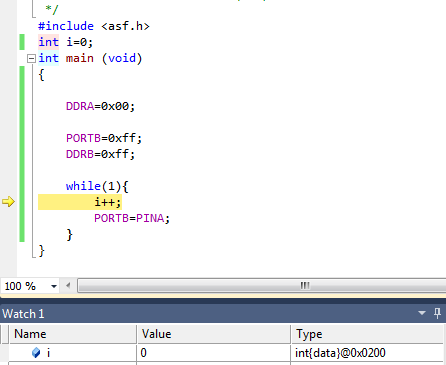
\includegraphics[scale=0.8]{MicroLab3/i_0}}
\caption{The first loop of the program i is still equal initialization value}
\end{figure}
There are a lot of useful tools provided for debugging, for example it is possible to follow the variables values through Watch window, Figure 1.\\\\
There is the first program loop before increment, variable i has an initial value 0.\\\\
Figure 2 shows us that the value became 1, after increment.
\begin{figure}[H]
\centerline{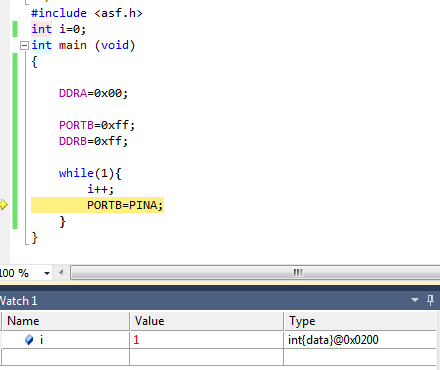
\includegraphics[scale=0.8]{MicroLab3/i_1}}
\caption{The end of the first loop of the program the variable was incremented}
\end{figure}
And the variable is again incremented in the second program loop.
\begin{figure}[H]
\centerline{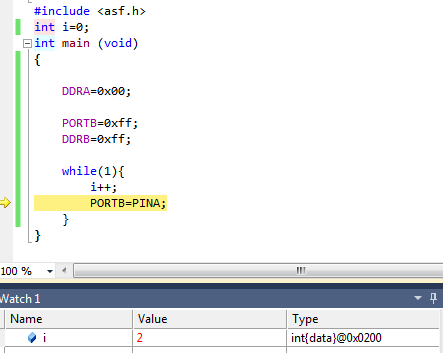
\includegraphics[scale=0.8]{MicroLab3/i_2}}
\caption{i was again incremented at the second loop}
\end{figure}
We also can see changes on the registers. When one of the switches is press the correspondent value in register was forced to change.
\begin{figure}[H]
\centerline{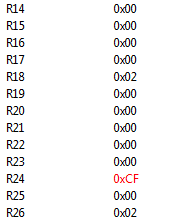
\includegraphics[scale=0.8]{MicroLab3/swithc_pressed}}
\caption{R24 was changed from 0x00 to 0xCF}
\end{figure}
When the button is released the value became initial value.

\section{Operating the IO pins}
\begin{figure}[H]
\centerline{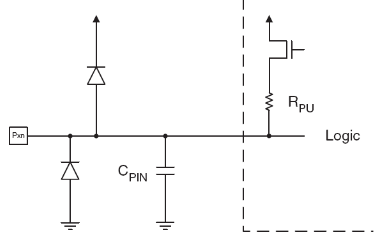
\includegraphics[scale=0.8]{MicroLab3/diagram}}
\caption{Diagram picture}
\end{figure}
In the figure there is written a general form of port pins for all AVR digital I/O ports. All of them have their individual selectable pull-up resistor with a supply-voltage invariant resistance, few protection diodes to both Vcc and Ground. There are three I/O memory address locations for each port: Data Register – PORTxn (Pxn), Data Direction Register – DDRx and Port Input Pins – PINx. A lower case “x” represents the port number, and a lower case “n” represents the bit number.\\\\
Example:\\\\
If we will define that PORTB (PORT[x] form) will handle LEDs, that means that each pin of port B (PB0, PB1, PB2, PB3, PB4, PB5, PB6, PB7) have each own Led accordingly LED port (LED0, LED1, LED2, LED3, LED4, LED5, LED6, LED7). If we setted SWITCHES to PORTA (PORT[x] form), that means that (PA0, PA1, PA2, PA3, PA4, PA5, PA6, PA7) configured to read a signal from switches (SW0, SW1, SW2, SW3, SW4, SW5, SW6, SW7) and write them to A register. And after that if we want to switch on the led with the same number as a number of pressed button, we have to read the data from PINA (PINx form) and set the value to the Data Register of Switches (PORTB).\\\\
 PORTB=PINA;//LedOn\\\\
Or in some cases we can select a necessary bit just calling that in this form: PORTB2\\\\
where we call the bit number 2 in PORTB Data Register.\\\\
Port Input Pins I/O location is only for reading, two other locations can be used for reading/writing.\\\\
However, writing a logic one to a bit in the PINx Register, will result in a toggle in the corresponding bit in the Data Register. In addition, the Pull-up Disable – PUD bit in MCUCR disables the pull-up function for all pins in all ports when set.
\section{Programs}

\subsection{The first program}
\begin{lstlisting}
#include <asf.h>
#include <util/delay.h>

#define SetBit(port, bit) {port = port &~( 1 << bit);}
#define ResetBit(port, bit) {port = port|( 1 << bit);}

void buttonsOnOff(int i);

int main (void)
{
	int i;
		board_init();
		DDRA = 0x00; 
		PORTB = 0xff;
		DDRB = 0xff; 	

	while(1)
	{		
	
			
	for(i=0;i<8;i++)
		buttonsOnOff(i);

	
	for(i=7;i>=0;i--)
		buttonsOnOff(i);	
	
}

}
void buttonsOnOff(int i){	
	int j,stopLoop=1;
		
		SetBit(PORTB,i);
	for(j=0;j<50;j++){		
		stopLoop=PINA!=0xff?-stopLoop:stopLoop;
		while(PINA!=0xff);
		while(stopLoop<0){
			stopLoop=PINA!=0xff?-stopLoop:stopLoop;
			while(PINA!=0xff);
		}
		_delay_ms(10);	
		}
	ResetBit(PORTB,i);	
}


\end{lstlisting}

\subsection{The second program}
\begin{lstlisting}
#include <asf.h>
#include <util/delay.h>

#define SetBit( port, bit) { port = port &~( 1 << bit); }
#define ResetBit( port, bit) { port = port|( 1 << bit); }

void AnotherWay(int i, int j);

void oneWay(int i, int j)
{
	int k;
	for(i=j;i<8;i++)
	{
		SetBit(PORTB,i);
		for(k=0;k<300;k++){
			if(PINA!=0xff){
				ResetBit(PORTB,i);
				while(PINA!=0xff);
				j=i;
				AnotherWay(i,j);
			}
			_delay_ms(10);
		}
		ResetBit(PORTB,i);
	}
	oneWay(0,0);
}

void AnotherWay(int i, int j)
{
	int k;
	if(j<0)
	j=8;
	for(i=j-1;i>=0;i--)
	{
		SetBit(PORTB,i);
		for(k=0;k<300;k++){			
			if(PINA!=0xff){
				ResetBit(PORTB,i);
				while(PINA!=0xff);
				j=i;
				oneWay(i,j);	
			}
			_delay_ms(10);
		}
		ResetBit(PORTB,i);
	}
	AnotherWay(8,8);
}

int main (void)
{
	int j=0,i=j;
		board_init();
		DDRA = 0x00; 
		PORTB = 0xff;
		DDRB = 0xff; 	
		oneWay(i,j);	
}


\end{lstlisting}
\subsection{The third program}
\begin{lstlisting}
#include <asf.h>
#include <util/delay.h>
#include <math.h>

#define F_CPU 16000000

int main (void)
{
	unsigned char bCounter=0;
		board_init();
			
		while(1)
			if(PINA!=0xff) // a key is pressed
			{
				bCounter++;
				while(PINA!=0xff); // wait until released
				PORTB=~bCounter;
			}
	   	   
	return 0;
}



//board_init

void board_init(void)
{
		DDRA = 0x00;  // input
		PORTA = 0xff; // pull up to 5V resistor to switch

		DDRB = 0xff;  // output for leds
		PORTB = 0xff; // turn off
}
\end{lstlisting}

\end{document}
